
The next set of performance analysis tools that we are going to learn about is the profiling tools, or profilers. We have already seen a profiler in use: in the last section, we used it to identify the function that was taking the majority of the computation time. This is exactly what profilers are used for, to find "hot" functions and code fragments, that is, the lines of code where the program spends the most time.

There are many different profiling tools available, both commercial and open source. In this section, we are going to examine two profilers that are popular on Linux systems. The goal is not to make you an expert on a particular tool but to give you an idea of what to expect from the profiler you choose to use and how to interpret its results.

First, let us point out that there are several different types of profilers:

\begin{itemize}
\item Some profilers execute the code under an interpreter or a virtual machine and observe where it spends the time. The main downside of these profilers is that they make the program run much slower than the code compiled directly to machine instructions, at least for languages like C++ that are so compiled and do not normally run under a virtual machine.

\item Other profilers require that the code is instrumented with special instructions during compilation or linking. These instructions provide additional information to the profiler, for example, so that they can notify the data collection engine when a function is called or a loop begins and ends. These profilers are faster than the ones of the previous type but still slower than the native execution. They also require a special compilation of the code and rely on the assumption that the instrumented code has the same performance as the original code, at least relatively, if not absolutely.

\item Most modern profilers use the hardware event counters that are present on all modern CPUs. These are special hardware registers that can be used to track certain hardware events. An example of a hardware event is executing an instruction. You can see how this can be useful for profiling: the processor will do the work of counting instructions for us without any additional instrumentation or any overhead. All we need to do is to read the values of the counter registers.

\end{itemize}

Unfortunately, useful profiling is a bit more complicated than simply counting instructions. We need to know how much time was spent in each function and even in each line of code. This can be done if the profiler reads the instruction count before and after executing each function (or each loop, each line of code, and so on). This is why some profilers use a hybrid approach: they instrument the code to mark the points of interest but use the hardware performance counters for the actual measurements.

Other profilers rely on time-based sampling: they interrupt the program at a certain interval, say, once per 10 milliseconds, and record the values of the performance counters as well as the current location of the program (the instruction that is about to be executed). If, say, 90\% of all samples were taken during a call to the compare() function, we can assume that the program spends 90\% of the time doing string comparisons. The accuracy of this approach depends on the number of samples taken and the interval between the samples.

The more often we sample the execution of the program, the more data we collect, but the greater the overhead is as well. Hardware-based profilers can, in some cases, have no adverse effect on the runtime of the program at all if the sampling is done not too often.

\subsubsubsection{2.4.1\hspace{0.2cm}The perf profiler}

The first profiler tool we are going to learn in this section is the Linux perf profiler. This is one of the most popular profilers on Linux simply because it comes installed with most distributions. This profiler uses hardware performance counters and time-based sampling; it does not require any instrumentation of the code. 

The simplest way to run this profiler is to collect the counter values for the entire program; this is done using the perf stat command:

\hspace*{\fill} \\ %插入空行
\begin{center}
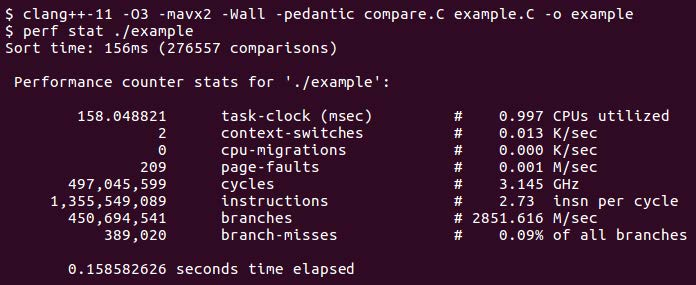
\includegraphics[width=0.9\textwidth]{content/1/chapter2/images/6.jpg}\\
Figure 2.6
\end{center}

As you can see in Figure 2.6, the compilation does not require any special options or tools. The program is executed by the profiler, and the stat option tells the profiler to display the counts accumulated in the hardware performance counters during the entire run of the program. In this case, our program ran for 158 milliseconds (consistent with the time printed by the program itself) and executed over 1.3 billion instructions. There are several other counters shown, such as "page-faults" and "branches." What are these counters, and what other counters can we see?

As it turns out, modern CPUs can collect statistics on many different types of events, but only a few types at a time; in the preceding example, eight counters were reported, so we can assume that this CPU has eight independent counters. However, each of these counters can be assigned to count one of many event types. The profiler itself can list all the events that are known to it and can be counted:

\hspace*{\fill} \\ %插入空行
\begin{center}
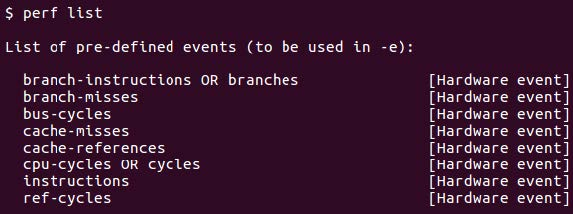
\includegraphics[width=0.9\textwidth]{content/1/chapter2/images/7.jpg}\\
Figure 2.7
\end{center}

The list in Figure 2.7 is incomplete (the printout continues for many more lines), and the exact counters available vary from one CPU to another (and, if you use a virtual machine, on the type and configuration of the hypervisor). The results collected by our profiling run in Figure 2.6 are simply the default set of counters, but we can select other counters for profiling:

\hspace*{\fill} \\ %插入空行
\begin{center}
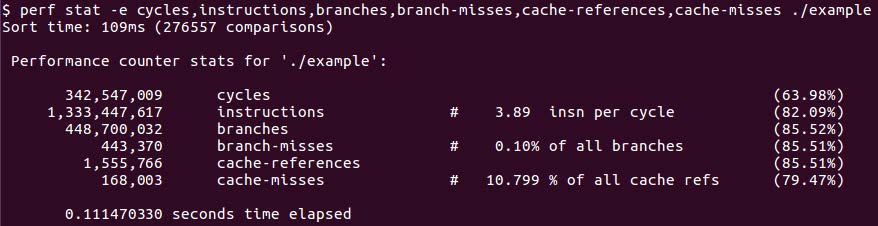
\includegraphics[width=0.9\textwidth]{content/1/chapter2/images/8.jpg}\\
Figure 2.8
\end{center}

In Figure 2.8, we measure CPU cycles and instructions, as well as branches, branch misses, cache references, and cache misses. A detailed explanation of these counters and the events they monitor will be presented in the next chapter.

Briefly, the cycle time is the inverse of the CPU frequency, so a 3GHz CPU can run 3 billion cycles per second. By the way, most CPUs can run at variable speeds, which complicates the measurements. Thus, for accurate profiling and benchmarking, it is recommended to disable the power saving mode and other features that can cause the CPU clock to vary. The instruction counter measures the number of processor instructions that were executed; as you can see, the CPU executes, on average, almost four instructions per cycle.

The "branches" are the conditional instructions: every if statement and every for loop with a condition generates at least one of these instructions. Branch misses will be explained in detail in the next chapter; for now, we can just say that it is an expensive and undesirable event, from the performance point of view.

The "cache references" count how many times the CPU needed to fetch something from memory. Most of the time, "something" is a piece of data, such as a character in the string. Depending on the state of the processor and memory, this fetch can be very fast or very slow; the latter is counted as a "cache miss" ("slow" is a relative concept; relative to the processor speed of 3 GHz, 1 microsecond is a very long time). The memory hierarchy will be explained in a later chapter; again, a cache miss is an expensive event. 

Armed with an understanding of how the CPUs and the memory work, you will be able to use such measurements to gauge the overall efficiency of your program and determine what kinds of factors are limiting its performance.

So far, we have seen only whole-program measurements. The measurements in Figure 2.8 may tell us what is holding back the performance of our code: for example, if we accept for now that "cache misses" are bad for performance, we can deduce that the main problem in this code is its inefficient memory access (one out of ten memory accesses is slow). However, this type of data does not tell us which parts of the code are responsible for poor performance. For that, we need to collect the data not just before and after but also during the program execution. Let us see how to do that with perf.

\subsubsubsection{2.4.2\hspace{0.2cm}Detailed profiling with perf}

The perf profiler combines the hardware counters with time interval-based sampling to record the profile of the running program. For each sample, it records the position of the program counter (the address of the instruction to be executed) and the values of the performance counters that we are monitoring. After the run, the data is analyzed; the functions and code lines with the most samples are responsible for the majority of the execution time.

The data collection run of the profiler is no more difficult than the overall measurement run. Note that, at run time, the instruction addresses are collected; to convert these to the line numbers in the original source code, the program must be compiled with debug information. If you are used to the two compilation modes, "optimized" and "debug non-optimized," this combination of compiler options may come as a surprise: both debug and optimization are enabled. The reason for the latter is that we need to profile the same code that will run in production, otherwise, the data is mostly meaningless. With this in mind, we can compile our code for profiling and run the profiler using the perf record command:

\hspace*{\fill} \\ %插入空行
\begin{center}
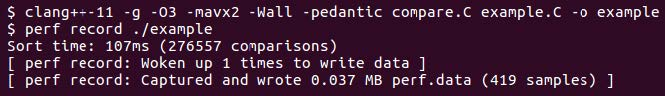
\includegraphics[width=0.9\textwidth]{content/1/chapter2/images/9.jpg}\\
Figure 2.9
\end{center}

Just like perf stat, we could have specified a counter or a set of counters to monitor but, this time, we accept the default counter. We haven't specified how often the samples are taken; again, there is a default for that, but we could also specify it explicitly: for example, perf record -c 1000 records 1000 samples per second.

The program runs, produces its regular output, as well as the messages from the profiler. The last one tells us that the profiling samples have been captured in the file named perf.data (again, this is the default that can be changed). To visualize the data from this file, we need to use the profile analysis tool, which is also a part of the same perftools suite, specifically, the perf report command. Running this command will launch this screen:

\hspace*{\fill} \\ %插入空行
\begin{center}
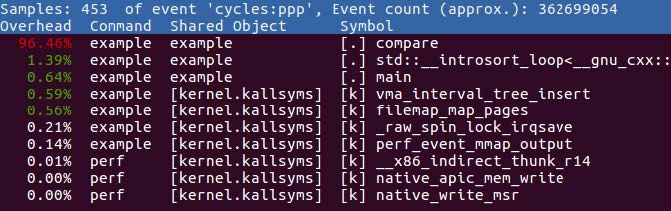
\includegraphics[width=0.9\textwidth]{content/1/chapter2/images/10.jpg}\\
Figure 2.10
\end{center}

This is the profiling summary, a breakdown of the execution time by function. From here, we can drill down into any function and see which lines contributed the most to the execution time:

\hspace*{\fill} \\ %插入空行
\begin{center}
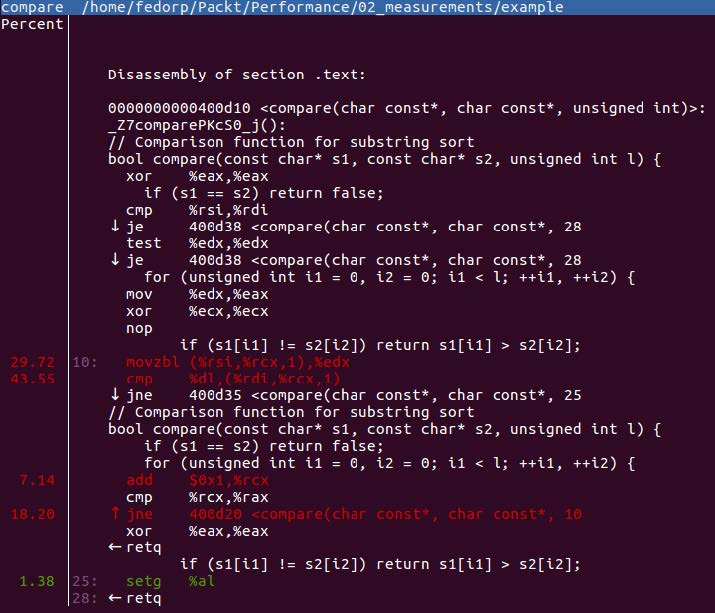
\includegraphics[width=0.9\textwidth]{content/1/chapter2/images/11.jpg}\\
Figure 2.11
\end{center}

The numbers on the left in Figure 2.11 are the percentages of the execution time spent at each line. So, what exactly does the "line" tell us? Figure 2.11 illustrates one of the more frequent difficulties in analyzing such profiles. It shows both the source code and the assembly instructions produced from it; the execution time counters are, naturally, associated with every hardware instruction (that is what the CPU executes, so that's the only thing it can count). The correspondence between the compiled code and the source is established by the profiler using the debugging information embedded by the compiler. Unfortunately, this correspondence is not exact, and the reason for this is optimization. The compiler performs a wide range of optimizations, all of which end up rearranging the code and changing the way the computations are done. You can see the results even in this very simple example: why does the source code line

\begin{lstlisting}[style=styleCXX]
if (s1 == s2) return false;
\end{lstlisting}

the instructions generated from this line are not all in the same place; the optimizer reordered them with the instructions originating from other lines. So the profiler shows this line near both machine instructions that were originally generated from it.

Even without looking at the assembler, we can see that the time is spent comparing the characters, as well as running the loop itself; these two source lines account for most of the time:

\begin{lstlisting}[style=styleCXX]
for (unsigned int i1 = 0, i2 = 0; i1 < l; ++i1, ++i2) {
	if (s1[i1] != s2[i2]) return s1[i1] > s2[i2];
\end{lstlisting}

To get the most out of the profile, it helps to understand at least the basics of the assembly language of the platform we're working on (X86 CPUs, in our case). The profiler also has some helpful tools that facilitate the analysis. For example, by placing the cursor on the jne (jump if not equal) instruction, we can see where the jump would take us, as well as the condition associated with the jump:

\hspace*{\fill} \\ %插入空行
\begin{center}
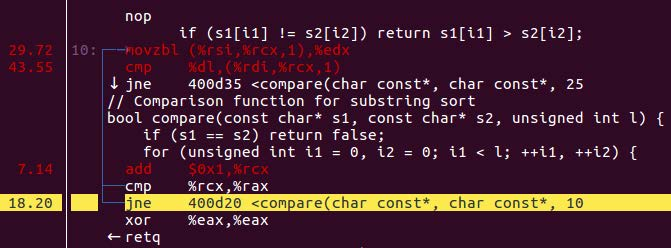
\includegraphics[width=0.9\textwidth]{content/1/chapter2/images/12.jpg}\\
Figure 2.12
\end{center}

This looks like a jump back to repeat the last few lines of code, so the cmp (compare) instruction above the jump must be the comparison of the loop, i1 < l. Together, the jump and the comparison account for 18\% of the execution time, so our earlier attention to the seemingly unnecessary comparison operation appears justified.

The perf profiler has many more options and capabilities for analyzing, filtering, and aggregating the results, all of which you can learn from its documentation. There are also several GUI frontends for this profiler. Next, we are going to take a quick look at another profiler, the one from Google Performance tools.

\subsubsubsection{2.4.3\hspace{0.2cm}The Google Performance profiler}

The Google CPU profiler also uses hardware performance counters. It also requires link-time instrumentation of the code (but no compile-time instrumentation). To prepare the code for profiling, you have to link it with the profiler library:

\hspace*{\fill} \\ %插入空行
\begin{center}

\includegraphics[width=0.9\textwidth]{content/1/chapter2/images/13.jpg}\\
Figure 2.13
\end{center}

In Figure 2.13, the library is specified by the command-line option –lprofiler. Unlike perf, this profiler does not need any special tools to invoke the program; the necessary code is already linked into the executable. The instrumented executable does not automatically start profiling itself. We have to activate the profiling by setting the environment variable CPUPROFILE to the filename of the file where we want to store the results. Other options are also controlled through the environment variables instead of command-line options, for example, the variable CPUPROFILE\_FREQUENCY sets the number of samples per second:

\hspace*{\fill} \\ %插入空行
\begin{center}
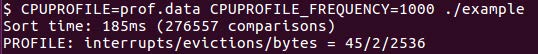
\includegraphics[width=0.9\textwidth]{content/1/chapter2/images/14.jpg}\\
Figure 2.14
\end{center}

Again, we see the output from the program itself and from the profiler, and we get the profile data file that we must analyze. The profiler has both the interactive and the batch mode; the interactive mode is a simple text user interface:

\hspace*{\fill} \\ %插入空行
\begin{center}
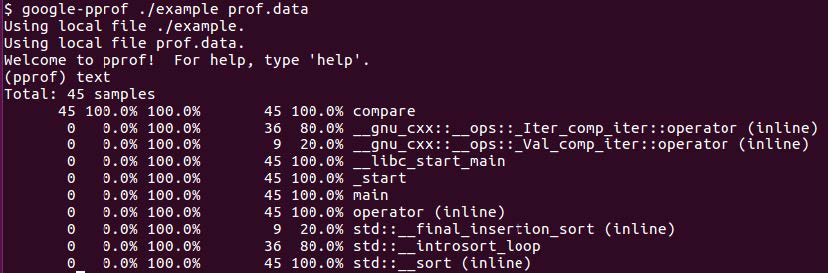
\includegraphics[width=0.9\textwidth]{content/1/chapter2/images/15.jpg}\\
Figure 2.15
\end{center}

Simply running google-pprof (often installed as just pprof) with the names of the executable and the profile as arguments brings up the command prompt. From here, we can, for example, get the summary of all functions annotated with percentages of the execution time. We can further analyze the program performance at the source code level:

\hspace*{\fill} \\ %插入空行
\begin{center}
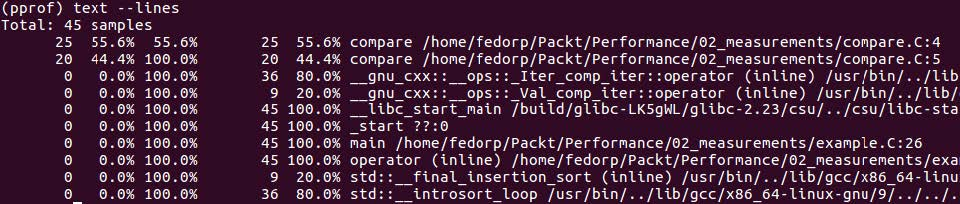
\includegraphics[width=0.9\textwidth]{content/1/chapter2/images/16.jpg}\\
Figure 2.16
\end{center}

As you can see, this profiler takes a slightly different approach and does not immediately dump us, neck-deep, into machine code (although annotated assembly can also be produced). This apparent simplicity is somewhat deceptive, though: the caveats we described earlier still apply, the optimizing compiler still does its transformations on the code.

Different profilers have somewhat different strengths and weaknesses, owing to the different approaches taken by their authors. Without turning this chapter into a profier manual, we will show in the rest of this section some of the more common problems you may encounter when collecting and analyzing the profile.

\subsubsubsection{2.4.4\hspace{0.2cm}Profiling with call graphs}

So far, our simple example has avoided one problem that, in reality, happens in every program. When we discovered that the comparison function is responsible for the majority of the execution time, we immediately knew which part of the program is responsible: there was only one line that calls this function.

Most real-life programs are not so simple: after all, one of the main reasons we write functions is to facilitate code reuse. It stands to reason that many functions will be called from multiple locations, some many times and others just a few times, often with very different parameters. Simply knowing which function takes a lot of time is not enough: we also need to know in which context it happens (after all, the most effective optimization may be to call the expensive function less often).

What we need is a profile that does not just tell us how much time is spent in each function and on each line of code, but also how much time is spent in each call chain. These profilers usually present this information using the call graphs: graphs where callers and callees are nodes and calls are edges.

First, we have to modify our example so we can call some function from more than one location. Let us start by making two sort calls:

\hspace*{\fill} \\ %插入空行
\noindent
\textbf{05\_compare\_timer.C}
\begin{lstlisting}[style=styleCXX]
std::sort(vs.begin(), vs.end(),
  [&](const char* a, const char* b) {
	++count; return compare1(a, b, L); });
std::sort(vs.begin(), vs.end(),
  [&](const char* a, const char* b) {
	++count; return compare2(a, b, L); });
\end{lstlisting}

The calls differ only in the comparison functions; in our case, the first comparison function is the same as before, and the second one produces the opposite order. The two functions have the same loop over substring characters as our old comparison function:

\hspace*{\fill} \\ %插入空行
\noindent
\textbf{05\_compare\_timer.C}
\begin{lstlisting}[style=styleCXX]
bool compare1(const char* s1, const char* s2, unsigned int l) {
	if (s1 == s2) return false;
	for (unsigned int i1 = 0, i2 = 0; i1 < l; ++i1, ++i2) {
		int res = compare(s1[i1], s2[i2]);
		if (res != 0) return res > 0;
	}
	return false;
}
bool compare2(const char* s1, const char* s2, unsigned int l) {
	if (s1 == s2) return false;
	for (unsigned int i1 = 0, i2 = 0; i1 < l; ++i1, ++i2) {
		int res = compare(s1[i1], s2[i2]);
		if (res != 0) return res < 0;
	}
	return false;
}
\end{lstlisting}

Both functions use the same common function to compare each character:

\begin{lstlisting}[style=styleCXX]
int compare(char c1, char c2) {
	if (c1 > c2) return 1;
	if (c1 < c2) return -1;
	return 0;
}
\end{lstlisting}

This isn't, of course, how you would do it in a real program: if you really wanted to avoid the code duplication caused by repeating the loop, you would write a single function parametrized by the character comparison operator. However, we do not want to deviate too far from the example we started with, and we want to keep the code simple so we can explain the results one complication at a time.

Now we are ready to produce a call graph that will show us how the cost of the character comparison is split between the two calls to sort. Both profilers we have used can produce call graphs; in this section, we will use the Google profiler. For this profiler, data collection already included the call chain information; we just haven't tried to visualize it so far.

We compile the code and run the profiler exactly as we did it earlier (for simplicity, we put each function in its own source file):

\hspace*{\fill} \\ %插入空行
\begin{center}
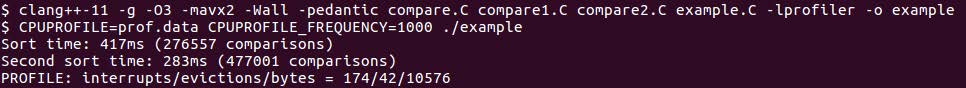
\includegraphics[width=0.9\textwidth]{content/1/chapter2/images/17.jpg}\\
Figure 2.17
\end{center}

The profiler can show the call graph in several different formats (Postscript, GIF, PDF, and so on). For example, to generate the PDF output, we would run this command:

\begin{tcblisting}{commandshell={}}
google-pprof --pdf ./example prof.data > prof.pdf
\end{tcblisting}

The information we're interested in right now is at the bottom of the call graph: 

\hspace*{\fill} \\ %插入空行
\begin{center}
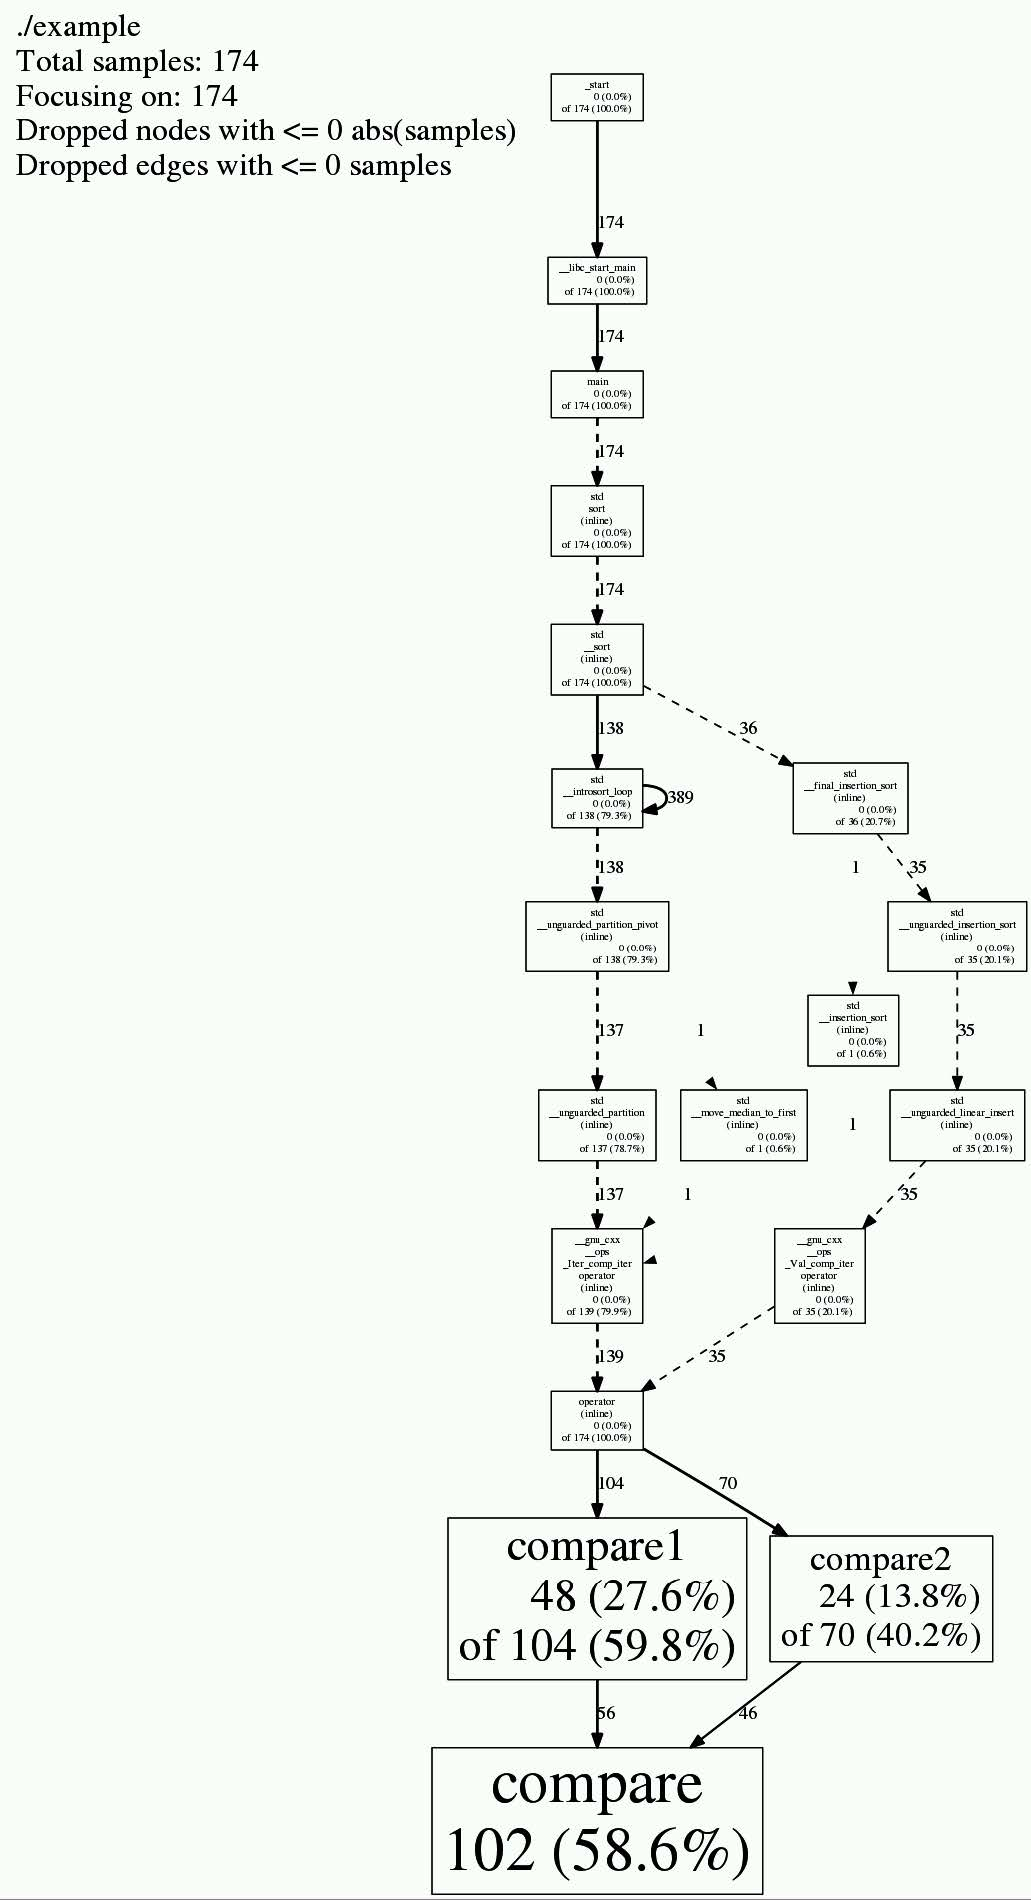
\includegraphics[width=0.9\textwidth]{content/1/chapter2/images/18.jpg}\\
Figure 2.18
\end{center}

As you can see in Figure 2.18, the compare() function, which accounts for 58.6\% of the total execution time, has two callers. Of the two, the compare1() function makes slightly more calls than the compare2() function; the former accounts for 27.6\% of the execution time (or 59.8\% if you include the time spent in its share of calls to compare()) and the latter is responsible for 13.8\% of the time by itself, or 40.2\% in total.

The basic call graphs are often enough to identify the problem call chains and select areas of the program for further exploration. Profiling tools also have more advanced reporting capabilities, such as the filtering of function names, aggregation of results, and so on. Mastering the features of your chosen tool can be the difference between knowledge and guesswork: interpreting performance profiles can be tricky and frustrating, and there are many reasons for it: some arise from tool limitations, but others are more fundamental. In the next section, we will talk about one of the latter reasons: for the measurements to be relevant, they must be done on fully optimized code.

\subsubsubsection{2.4.5\hspace{0.2cm}Optimization and inlining}

We have already seen how compiler optimization muddies the waters when it comes to interpreting performance profiles: all profiling is done, at the end of the day, on the compiled machine code, while we see the program in its source form. The relation between these two forms is obscured by compiler optimizations. One of the most aggressive optimizations, in terms of rearranging the source code, is compile-time inlining of function calls.

The inlining requires that the source of the function be visible at the call site, so, in order to show you how this looks, we have to combine the entire source code in one file:+

\hspace*{\fill} \\ %插入空行
\noindent
\textbf{02\_substring\_sort.C}
\begin{lstlisting}[style=styleCXX]
bool compare(const char* s1, const char* s2, unsigned int l) {
	if (s1 == s2) return false;
	for (unsigned int i1 = 0, i2 = 0; i1 < l; ++i1, ++i2) {
		if (s1[i1] != s2[i2]) return s1[i1] > s2[i2];
	}
	return false;
}
int main() {
	…
	size_t count = 0;
	std::sort(vs.begin(), vs.end(),
	  [&](const char* a, const char* b) {
		++count; return compare(a, b, L); });
}
\end{lstlisting}

Now the compiler can, and probably will, generate the machine code for the comparison right where it is used by the sort, instead of calling the external function. Such inlining is a potent optimization tool; it happens quite often and not just with functions from the same file. Much more often, inlining affects header-only functions (functions whose entire implementation is in the header file). For example, in the preceding code, the call to std::sort, which looks like a function call, is almost certainly inlined because std::sort is a template function: its entire body is in the header files.

Let us see how the profiler tools we used earlier deal with the inlined code. Running the Google profiler for annotated source lines produces this report:

\hspace*{\fill} \\ %插入空行
\begin{center}
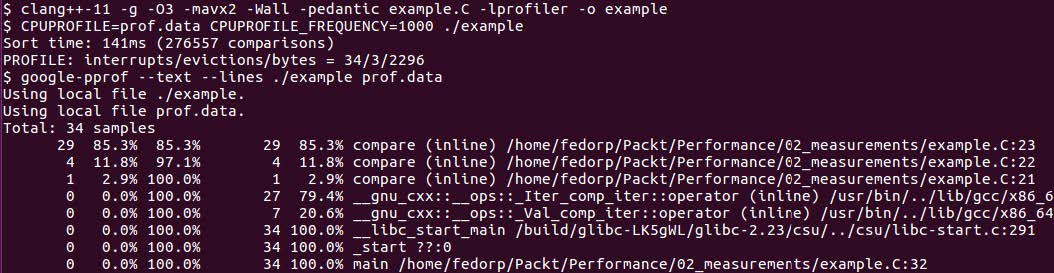
\includegraphics[width=0.9\textwidth]{content/1/chapter2/images/19.jpg}\\
Figure 2.19
\end{center}

As you can see, the profiler knows that the compare() function was inlined but still shows its original name. The lines in the source code correspond to the location where the code for the function is written, not where it is called, for example, line 23 is this line:

\begin{lstlisting}[style=styleCXX]
if (s1[i1] != s2[i2]) return s1[i1] > s2[i2];
\end{lstlisting}

The perf profiler, on the other hand, does not show inline functions as easily:

\hspace*{\fill} \\ %插入空行
\begin{center}
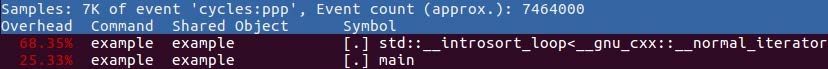
\includegraphics[width=0.9\textwidth]{content/1/chapter2/images/20.jpg}\\
Figure 2.20
\end{center}

Here we can see that the time appears to be spent in the sort code and the main program itself. Examining the annotated source, however, shows us that the code that was generated from the compare() function's source is still responsible for the absolute majority of the execution time:

\hspace*{\fill} \\ %插入空行
\begin{center}
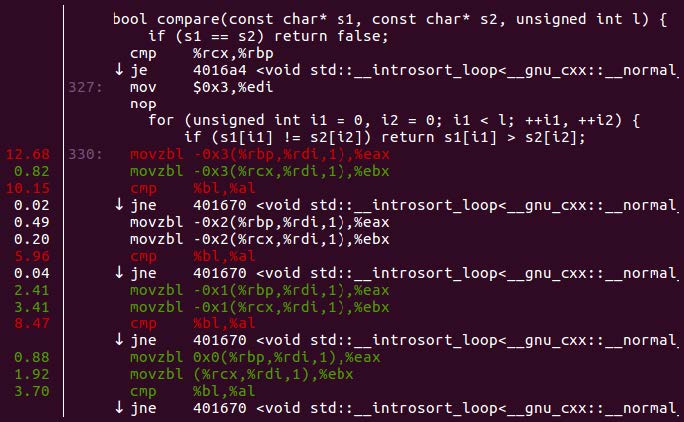
\includegraphics[width=0.9\textwidth]{content/1/chapter2/images/21.jpg}\\
Figure 2.21
\end{center}

There is, unfortunately, no easy way to undo the effects of the optimizations on the performance profiles. Inlining, code reordering, and other transformations turn detailed performance analysis into a skill that develops with practice. Perforce, some practical suggestions for the effective use of profiling are now in order.

\subsubsubsection{2.4.6\hspace{0.2cm}Practical profiling}

It may be tempting to think of profiling as the ultimate solution to all your performance measurement needs: run the whole program under a profiler, collect all the data, and get the complete analysis of everything that is going on in the code. Unfortunately, it rarely works out this way. Sometimes, the tool limitations get in the way. Often, the complexity of the information contained in the large amounts of data is simply too overwhelming. How, then, should you use profiling effectively?

The recommended approach is to collect high-level information first, then refine it. A coarse profile that breaks down the execution time between large modules may be a good place to start. On the other hand, you may have that information already if the modules are instrumented for benchmarking and have timers bracketing all major execution steps. If you don't have such instrumentation, the initial profile offers good suggestions for what these steps are, so consider adding the benchmarking instrumentation now, so you have them next time: you don't really expect to solve all your performance problems once and for all, do you?

With the benchmarking results and the coarse profile, you will likely encounter one of several scenarios. If you are very lucky, the profile will point to some low-hanging fruit, like a function that takes 99\% of the time doing a sort of a list. Yes, it happens: nobody expected the list to be longer than ten elements when the code was first written, and so it was for a while, and then everyone forgot about that code until it showed up as the long pole on the profile.

More likely, the profile will lead you to some large functions or modules. Now you have to iterate, create tests that focus on the interesting parts of the program, and profile a smaller portion of the code in more detail. Some amount of benchmarking data can also be very helpful in interpreting the profiles: while the profile will tell you how much time was spent in a given function or a loop, it won't count loop iterations or trace through if-else conditions. Note that most profilers can count function calls, so a good modular code is easier to profile than a huge monolithic mess.

As you collect and refine the profiles, the data will guide your attention toward the performance-critical areas of the code. It is also the point where you can fall into a common error: as you are focused on the code that is too slow, you may jump to optimizing it without considering the bigger picture. For example, the profile shows that a particular loop spends most time in memory allocation. Before you decide that you need a more efficient memory allocator, consider whether you actually need to allocate and deallocate memory on every iteration of the loop. The best way to make slow code faster is often to call it less often. This may require a different algorithm or just a more efficient implementation.

Just as often, you will discover that there is a computation you must do, it is the performance-critical part of the code, and the only way to speed up the program is to make this code faster. Now you have to try different ideas for optimizing it and see what works best. You can do it live in the program itself, but often this is a wasteful approach that significantly reduces your productivity. Ideally, you want to quickly experiment with different implementations or even different algorithms for a particular problem. It is here that you can take advantage of the third method for collecting performance data, microbenchmarking.













